% Created by tikzDevice version 0.12.6 on 2026-08-12 08:54:30
% !TEX encoding = UTF-8 Unicode
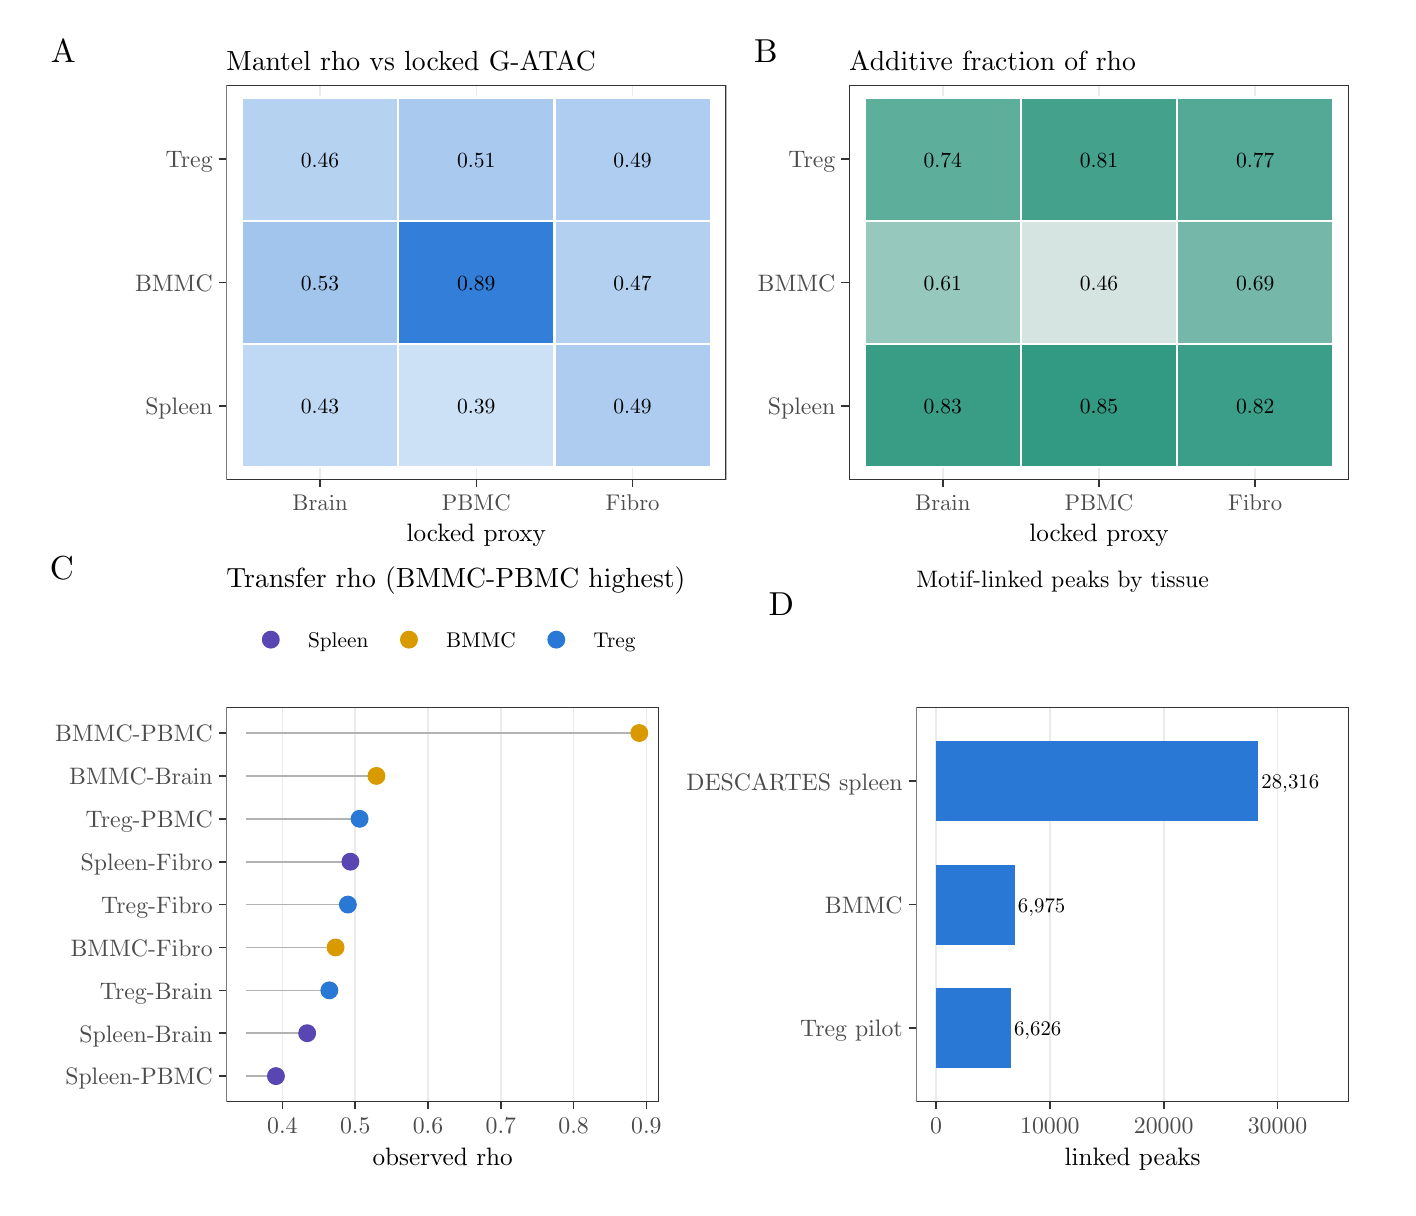
\begin{tikzpicture}[x=1pt,y=1pt]
\definecolor{fillColor}{RGB}{255,255,255}
\path[use as bounding box,fill=fillColor,fill opacity=0.00] (0,0) rectangle (491.44,419.17);
\begin{scope}
\path[clip] (  0.00,  0.00) rectangle (491.44,419.17);
\definecolor{drawColor}{RGB}{255,255,255}
\definecolor{fillColor}{RGB}{255,255,255}

\path[draw=drawColor,line width= 0.6pt,line join=round,line cap=round,fill=fillColor] ( -0.00,  0.00) rectangle (491.44,419.17);
\end{scope}
\begin{scope}
\path[clip] (  4.00,228.25) rectangle (258.43,415.17);
\definecolor{drawColor}{RGB}{255,255,255}
\definecolor{fillColor}{RGB}{255,255,255}

\path[draw=drawColor,line width= 0.6pt,line join=round,line cap=round,fill=fillColor] (  4.00,228.25) rectangle (258.43,415.17);
\end{scope}
\begin{scope}
\path[clip] (258.43,228.25) rectangle (485.44,415.17);
\definecolor{drawColor}{RGB}{255,255,255}
\definecolor{fillColor}{RGB}{255,255,255}

\path[draw=drawColor,line width= 0.6pt,line join=round,line cap=round,fill=fillColor] (258.43,228.25) rectangle (485.44,415.17);
\end{scope}
\begin{scope}
\path[clip] ( 71.81,255.84) rectangle (252.43,398.39);
\definecolor{fillColor}{RGB}{255,255,255}

\path[fill=fillColor] ( 71.81,255.84) rectangle (252.43,398.39);
\definecolor{drawColor}{gray}{0.92}

\path[draw=drawColor,line width= 0.6pt,line join=round] (105.67,255.84) --
	(105.67,398.39);

\path[draw=drawColor,line width= 0.6pt,line join=round] (162.12,255.84) --
	(162.12,398.39);

\path[draw=drawColor,line width= 0.6pt,line join=round] (218.56,255.84) --
	(218.56,398.39);
\definecolor{drawColor}{RGB}{255,255,255}
\definecolor{fillColor}{RGB}{191,216,243}

\path[draw=drawColor,line width= 0.8pt,fill=fillColor] ( 77.45,260.29) rectangle (133.90,304.84);
\definecolor{fillColor}{RGB}{204,224,246}

\path[draw=drawColor,line width= 0.8pt,fill=fillColor] (133.90,260.29) rectangle (190.34,304.84);
\definecolor{fillColor}{RGB}{173,204,239}

\path[draw=drawColor,line width= 0.8pt,fill=fillColor] (190.34,260.29) rectangle (246.79,304.84);
\definecolor{fillColor}{RGB}{162,197,237}

\path[draw=drawColor,line width= 0.8pt,fill=fillColor] ( 77.45,304.84) rectangle (133.90,349.39);
\definecolor{fillColor}{RGB}{51,126,216}

\path[draw=drawColor,line width= 0.8pt,fill=fillColor] (133.90,304.84) rectangle (190.34,349.39);
\definecolor{fillColor}{RGB}{179,208,241}

\path[draw=drawColor,line width= 0.8pt,fill=fillColor] (190.34,304.84) rectangle (246.79,349.39);
\definecolor{fillColor}{RGB}{182,210,241}

\path[draw=drawColor,line width= 0.8pt,fill=fillColor] ( 77.45,349.39) rectangle (133.90,393.94);
\definecolor{fillColor}{RGB}{169,201,239}

\path[draw=drawColor,line width= 0.8pt,fill=fillColor] (133.90,349.39) rectangle (190.34,393.94);
\definecolor{fillColor}{RGB}{174,205,240}

\path[draw=drawColor,line width= 0.8pt,fill=fillColor] (190.34,349.39) rectangle (246.79,393.94);
\definecolor{drawColor}{RGB}{0,0,0}

\node[text=drawColor,anchor=base,inner sep=0pt, outer sep=0pt, scale=  0.78] at (105.67,279.69) {0.43};

\node[text=drawColor,anchor=base,inner sep=0pt, outer sep=0pt, scale=  0.78] at (162.12,279.69) {0.39};

\node[text=drawColor,anchor=base,inner sep=0pt, outer sep=0pt, scale=  0.78] at (218.56,279.69) {0.49};

\node[text=drawColor,anchor=base,inner sep=0pt, outer sep=0pt, scale=  0.78] at (105.67,324.24) {0.53};

\node[text=drawColor,anchor=base,inner sep=0pt, outer sep=0pt, scale=  0.78] at (162.12,324.24) {0.89};

\node[text=drawColor,anchor=base,inner sep=0pt, outer sep=0pt, scale=  0.78] at (218.56,324.24) {0.47};

\node[text=drawColor,anchor=base,inner sep=0pt, outer sep=0pt, scale=  0.78] at (105.67,368.79) {0.46};

\node[text=drawColor,anchor=base,inner sep=0pt, outer sep=0pt, scale=  0.78] at (162.12,368.79) {0.51};

\node[text=drawColor,anchor=base,inner sep=0pt, outer sep=0pt, scale=  0.78] at (218.56,368.79) {0.49};
\definecolor{drawColor}{gray}{0.20}

\path[draw=drawColor,line width= 0.6pt,line join=round,line cap=round] ( 71.81,255.84) rectangle (252.43,398.39);
\end{scope}
\begin{scope}
\path[clip] (  0.00,  0.00) rectangle (491.44,419.17);
\definecolor{drawColor}{gray}{0.30}

\node[text=drawColor,anchor=base east,inner sep=0pt, outer sep=0pt, scale=  0.86] at ( 66.86,279.37) {Spleen};

\node[text=drawColor,anchor=base east,inner sep=0pt, outer sep=0pt, scale=  0.86] at ( 66.86,323.92) {BMMC};

\node[text=drawColor,anchor=base east,inner sep=0pt, outer sep=0pt, scale=  0.86] at ( 66.86,368.47) {Treg};
\end{scope}
\begin{scope}
\path[clip] (  0.00,  0.00) rectangle (491.44,419.17);
\definecolor{drawColor}{gray}{0.20}

\path[draw=drawColor,line width= 0.6pt,line join=round] ( 69.06,282.56) --
	( 71.81,282.56);

\path[draw=drawColor,line width= 0.6pt,line join=round] ( 69.06,327.11) --
	( 71.81,327.11);

\path[draw=drawColor,line width= 0.6pt,line join=round] ( 69.06,371.66) --
	( 71.81,371.66);
\end{scope}
\begin{scope}
\path[clip] (  0.00,  0.00) rectangle (491.44,419.17);
\definecolor{drawColor}{gray}{0.20}

\path[draw=drawColor,line width= 0.6pt,line join=round] (105.67,253.09) --
	(105.67,255.84);

\path[draw=drawColor,line width= 0.6pt,line join=round] (162.12,253.09) --
	(162.12,255.84);

\path[draw=drawColor,line width= 0.6pt,line join=round] (218.56,253.09) --
	(218.56,255.84);
\end{scope}
\begin{scope}
\path[clip] (  0.00,  0.00) rectangle (491.44,419.17);
\definecolor{drawColor}{gray}{0.30}

\node[text=drawColor,anchor=base,inner sep=0pt, outer sep=0pt, scale=  0.82] at (105.67,244.83) {Brain};

\node[text=drawColor,anchor=base,inner sep=0pt, outer sep=0pt, scale=  0.82] at (162.12,244.83) {PBMC};

\node[text=drawColor,anchor=base,inner sep=0pt, outer sep=0pt, scale=  0.82] at (218.56,244.83) {Fibro};
\end{scope}
\begin{scope}
\path[clip] (  0.00,  0.00) rectangle (491.44,419.17);
\definecolor{drawColor}{RGB}{0,0,0}

\node[text=drawColor,anchor=base,inner sep=0pt, outer sep=0pt, scale=  0.91] at (162.12,233.41) {locked proxy};
\end{scope}
\begin{scope}
\path[clip] (  0.00,  0.00) rectangle (491.44,419.17);
\definecolor{drawColor}{RGB}{0,0,0}

\node[text=drawColor,anchor=base west,inner sep=0pt, outer sep=0pt, scale=  1.00] at ( 71.81,403.76) {Mantel rho vs locked G-ATAC};
\end{scope}
\begin{scope}
\path[clip] (  0.00,  0.00) rectangle (491.44,419.17);
\definecolor{drawColor}{RGB}{0,0,0}

\node[text=drawColor,anchor=base,inner sep=0pt, outer sep=0pt, scale=  1.20] at ( 12.89,406.72) {A};
\end{scope}
\begin{scope}
\path[clip] (296.81,255.84) rectangle (477.44,398.39);
\definecolor{fillColor}{RGB}{255,255,255}

\path[fill=fillColor] (296.81,255.84) rectangle (477.44,398.39);
\definecolor{drawColor}{gray}{0.92}

\path[draw=drawColor,line width= 0.6pt,line join=round] (330.68,255.84) --
	(330.68,398.39);

\path[draw=drawColor,line width= 0.6pt,line join=round] (387.12,255.84) --
	(387.12,398.39);

\path[draw=drawColor,line width= 0.6pt,line join=round] (443.57,255.84) --
	(443.57,398.39);
\definecolor{drawColor}{RGB}{255,255,255}
\definecolor{fillColor}{RGB}{57,157,134}

\path[draw=drawColor,line width= 0.8pt,fill=fillColor] (302.46,260.29) rectangle (358.90,304.84);
\definecolor{fillColor}{RGB}{50,153,130}

\path[draw=drawColor,line width= 0.8pt,fill=fillColor] (358.90,260.29) rectangle (415.35,304.84);
\definecolor{fillColor}{RGB}{59,158,136}

\path[draw=drawColor,line width= 0.8pt,fill=fillColor] (415.35,260.29) rectangle (471.79,304.84);
\definecolor{fillColor}{RGB}{151,200,189}

\path[draw=drawColor,line width= 0.8pt,fill=fillColor] (302.46,304.84) rectangle (358.90,349.39);
\definecolor{fillColor}{RGB}{214,228,225}

\path[draw=drawColor,line width= 0.8pt,fill=fillColor] (358.90,304.84) rectangle (415.35,349.39);
\definecolor{fillColor}{RGB}{117,184,169}

\path[draw=drawColor,line width= 0.8pt,fill=fillColor] (415.35,304.84) rectangle (471.79,349.39);
\definecolor{fillColor}{RGB}{94,174,156}

\path[draw=drawColor,line width= 0.8pt,fill=fillColor] (302.46,349.39) rectangle (358.90,393.94);
\definecolor{fillColor}{RGB}{67,161,140}

\path[draw=drawColor,line width= 0.8pt,fill=fillColor] (358.90,349.39) rectangle (415.35,393.94);
\definecolor{fillColor}{RGB}{84,169,150}

\path[draw=drawColor,line width= 0.8pt,fill=fillColor] (415.35,349.39) rectangle (471.79,393.94);
\definecolor{drawColor}{RGB}{0,0,0}

\node[text=drawColor,anchor=base,inner sep=0pt, outer sep=0pt, scale=  0.78] at (330.68,279.69) {0.83};

\node[text=drawColor,anchor=base,inner sep=0pt, outer sep=0pt, scale=  0.78] at (387.12,279.69) {0.85};

\node[text=drawColor,anchor=base,inner sep=0pt, outer sep=0pt, scale=  0.78] at (443.57,279.69) {0.82};

\node[text=drawColor,anchor=base,inner sep=0pt, outer sep=0pt, scale=  0.78] at (330.68,324.24) {0.61};

\node[text=drawColor,anchor=base,inner sep=0pt, outer sep=0pt, scale=  0.78] at (387.12,324.24) {0.46};

\node[text=drawColor,anchor=base,inner sep=0pt, outer sep=0pt, scale=  0.78] at (443.57,324.24) {0.69};

\node[text=drawColor,anchor=base,inner sep=0pt, outer sep=0pt, scale=  0.78] at (330.68,368.79) {0.74};

\node[text=drawColor,anchor=base,inner sep=0pt, outer sep=0pt, scale=  0.78] at (387.12,368.79) {0.81};

\node[text=drawColor,anchor=base,inner sep=0pt, outer sep=0pt, scale=  0.78] at (443.57,368.79) {0.77};
\definecolor{drawColor}{gray}{0.20}

\path[draw=drawColor,line width= 0.6pt,line join=round,line cap=round] (296.81,255.84) rectangle (477.44,398.39);
\end{scope}
\begin{scope}
\path[clip] (  0.00,  0.00) rectangle (491.44,419.17);
\definecolor{drawColor}{gray}{0.30}

\node[text=drawColor,anchor=base east,inner sep=0pt, outer sep=0pt, scale=  0.86] at (291.86,279.37) {Spleen};

\node[text=drawColor,anchor=base east,inner sep=0pt, outer sep=0pt, scale=  0.86] at (291.86,323.92) {BMMC};

\node[text=drawColor,anchor=base east,inner sep=0pt, outer sep=0pt, scale=  0.86] at (291.86,368.47) {Treg};
\end{scope}
\begin{scope}
\path[clip] (  0.00,  0.00) rectangle (491.44,419.17);
\definecolor{drawColor}{gray}{0.20}

\path[draw=drawColor,line width= 0.6pt,line join=round] (294.06,282.56) --
	(296.81,282.56);

\path[draw=drawColor,line width= 0.6pt,line join=round] (294.06,327.11) --
	(296.81,327.11);

\path[draw=drawColor,line width= 0.6pt,line join=round] (294.06,371.66) --
	(296.81,371.66);
\end{scope}
\begin{scope}
\path[clip] (  0.00,  0.00) rectangle (491.44,419.17);
\definecolor{drawColor}{gray}{0.20}

\path[draw=drawColor,line width= 0.6pt,line join=round] (330.68,253.09) --
	(330.68,255.84);

\path[draw=drawColor,line width= 0.6pt,line join=round] (387.12,253.09) --
	(387.12,255.84);

\path[draw=drawColor,line width= 0.6pt,line join=round] (443.57,253.09) --
	(443.57,255.84);
\end{scope}
\begin{scope}
\path[clip] (  0.00,  0.00) rectangle (491.44,419.17);
\definecolor{drawColor}{gray}{0.30}

\node[text=drawColor,anchor=base,inner sep=0pt, outer sep=0pt, scale=  0.82] at (330.68,244.83) {Brain};

\node[text=drawColor,anchor=base,inner sep=0pt, outer sep=0pt, scale=  0.82] at (387.12,244.83) {PBMC};

\node[text=drawColor,anchor=base,inner sep=0pt, outer sep=0pt, scale=  0.82] at (443.57,244.83) {Fibro};
\end{scope}
\begin{scope}
\path[clip] (  0.00,  0.00) rectangle (491.44,419.17);
\definecolor{drawColor}{RGB}{0,0,0}

\node[text=drawColor,anchor=base,inner sep=0pt, outer sep=0pt, scale=  0.91] at (387.12,233.41) {locked proxy};
\end{scope}
\begin{scope}
\path[clip] (  0.00,  0.00) rectangle (491.44,419.17);
\definecolor{drawColor}{RGB}{0,0,0}

\node[text=drawColor,anchor=base west,inner sep=0pt, outer sep=0pt, scale=  1.00] at (296.81,403.76) {Additive fraction of rho};
\end{scope}
\begin{scope}
\path[clip] (  0.00,  0.00) rectangle (491.44,419.17);
\definecolor{drawColor}{RGB}{0,0,0}

\node[text=drawColor,anchor=base,inner sep=0pt, outer sep=0pt, scale=  1.20] at (266.73,406.72) {B};
\end{scope}
\begin{scope}
\path[clip] (  4.00,  3.00) rectangle (234.11,228.25);
\definecolor{drawColor}{RGB}{255,255,255}
\definecolor{fillColor}{RGB}{255,255,255}

\path[draw=drawColor,line width= 0.6pt,line join=round,line cap=round,fill=fillColor] (  4.00,  3.00) rectangle (234.11,228.25);
\end{scope}
\begin{scope}
\path[clip] (234.11,  3.00) rectangle (485.44,228.25);
\definecolor{drawColor}{RGB}{255,255,255}
\definecolor{fillColor}{RGB}{255,255,255}

\path[draw=drawColor,line width= 0.6pt,line join=round,line cap=round,fill=fillColor] (234.11,  3.00) rectangle (485.44,228.25);
\end{scope}
\begin{scope}
\path[clip] ( 71.81, 31.02) rectangle (228.11,173.58);
\definecolor{fillColor}{RGB}{255,255,255}

\path[fill=fillColor] ( 71.81, 31.02) rectangle (228.11,173.58);
\definecolor{drawColor}{gray}{0.92}

\path[draw=drawColor,line width= 0.6pt,line join=round] ( 92.06, 31.02) --
	( 92.06,173.58);

\path[draw=drawColor,line width= 0.6pt,line join=round] (118.36, 31.02) --
	(118.36,173.58);

\path[draw=drawColor,line width= 0.6pt,line join=round] (144.66, 31.02) --
	(144.66,173.58);

\path[draw=drawColor,line width= 0.6pt,line join=round] (170.97, 31.02) --
	(170.97,173.58);

\path[draw=drawColor,line width= 0.6pt,line join=round] (197.27, 31.02) --
	(197.27,173.58);

\path[draw=drawColor,line width= 0.6pt,line join=round] (223.57, 31.02) --
	(223.57,173.58);
\definecolor{drawColor}{gray}{0.70}

\path[draw=drawColor,line width= 0.6pt,line join=round] ( 78.91, 55.82) -- (100.99, 55.82);

\path[draw=drawColor,line width= 0.6pt,line join=round] ( 78.91, 40.32) -- ( 89.71, 40.32);

\path[draw=drawColor,line width= 0.6pt,line join=round] ( 78.91,117.80) -- (116.62,117.80);

\path[draw=drawColor,line width= 0.6pt,line join=round] ( 78.91,148.79) -- (126.02,148.79);

\path[draw=drawColor,line width= 0.6pt,line join=round] ( 78.91,164.29) -- (221.00,164.29);

\path[draw=drawColor,line width= 0.6pt,line join=round] ( 78.91, 86.81) -- (111.26, 86.81);

\path[draw=drawColor,line width= 0.6pt,line join=round] ( 78.91, 71.31) -- (109.01, 71.31);

\path[draw=drawColor,line width= 0.6pt,line join=round] ( 78.91,133.29) -- (119.94,133.29);

\path[draw=drawColor,line width= 0.6pt,line join=round] ( 78.91,102.30) -- (115.70,102.30);
\definecolor{drawColor}{RGB}{89,70,178}
\definecolor{fillColor}{RGB}{89,70,178}

\path[draw=drawColor,line width= 0.4pt,line join=round,line cap=round,fill=fillColor] (100.99, 55.82) circle (  3.03);

\path[draw=drawColor,line width= 0.4pt,line join=round,line cap=round,fill=fillColor] ( 89.71, 40.32) circle (  3.03);

\path[draw=drawColor,line width= 0.4pt,line join=round,line cap=round,fill=fillColor] (116.62,117.80) circle (  3.03);
\definecolor{drawColor}{RGB}{217,154,0}
\definecolor{fillColor}{RGB}{217,154,0}

\path[draw=drawColor,line width= 0.4pt,line join=round,line cap=round,fill=fillColor] (126.02,148.79) circle (  3.03);

\path[draw=drawColor,line width= 0.4pt,line join=round,line cap=round,fill=fillColor] (221.00,164.29) circle (  3.03);

\path[draw=drawColor,line width= 0.4pt,line join=round,line cap=round,fill=fillColor] (111.26, 86.81) circle (  3.03);
\definecolor{drawColor}{RGB}{42,120,214}
\definecolor{fillColor}{RGB}{42,120,214}

\path[draw=drawColor,line width= 0.4pt,line join=round,line cap=round,fill=fillColor] (109.01, 71.31) circle (  3.03);

\path[draw=drawColor,line width= 0.4pt,line join=round,line cap=round,fill=fillColor] (119.94,133.29) circle (  3.03);

\path[draw=drawColor,line width= 0.4pt,line join=round,line cap=round,fill=fillColor] (115.70,102.30) circle (  3.03);
\definecolor{drawColor}{gray}{0.20}

\path[draw=drawColor,line width= 0.6pt,line join=round,line cap=round] ( 71.81, 31.02) rectangle (228.11,173.58);
\end{scope}
\begin{scope}
\path[clip] (  0.00,  0.00) rectangle (491.44,419.17);
\definecolor{drawColor}{gray}{0.30}

\node[text=drawColor,anchor=base east,inner sep=0pt, outer sep=0pt, scale=  0.86] at ( 66.86, 37.13) {Spleen-PBMC};

\node[text=drawColor,anchor=base east,inner sep=0pt, outer sep=0pt, scale=  0.86] at ( 66.86, 52.62) {Spleen-Brain};

\node[text=drawColor,anchor=base east,inner sep=0pt, outer sep=0pt, scale=  0.86] at ( 66.86, 68.12) {Treg-Brain};

\node[text=drawColor,anchor=base east,inner sep=0pt, outer sep=0pt, scale=  0.86] at ( 66.86, 83.61) {BMMC-Fibro};

\node[text=drawColor,anchor=base east,inner sep=0pt, outer sep=0pt, scale=  0.86] at ( 66.86, 99.11) {Treg-Fibro};

\node[text=drawColor,anchor=base east,inner sep=0pt, outer sep=0pt, scale=  0.86] at ( 66.86,114.60) {Spleen-Fibro};

\node[text=drawColor,anchor=base east,inner sep=0pt, outer sep=0pt, scale=  0.86] at ( 66.86,130.10) {Treg-PBMC};

\node[text=drawColor,anchor=base east,inner sep=0pt, outer sep=0pt, scale=  0.86] at ( 66.86,145.59) {BMMC-Brain};

\node[text=drawColor,anchor=base east,inner sep=0pt, outer sep=0pt, scale=  0.86] at ( 66.86,161.09) {BMMC-PBMC};
\end{scope}
\begin{scope}
\path[clip] (  0.00,  0.00) rectangle (491.44,419.17);
\definecolor{drawColor}{gray}{0.20}

\path[draw=drawColor,line width= 0.6pt,line join=round] ( 69.06, 40.32) --
	( 71.81, 40.32);

\path[draw=drawColor,line width= 0.6pt,line join=round] ( 69.06, 55.82) --
	( 71.81, 55.82);

\path[draw=drawColor,line width= 0.6pt,line join=round] ( 69.06, 71.31) --
	( 71.81, 71.31);

\path[draw=drawColor,line width= 0.6pt,line join=round] ( 69.06, 86.81) --
	( 71.81, 86.81);

\path[draw=drawColor,line width= 0.6pt,line join=round] ( 69.06,102.30) --
	( 71.81,102.30);

\path[draw=drawColor,line width= 0.6pt,line join=round] ( 69.06,117.80) --
	( 71.81,117.80);

\path[draw=drawColor,line width= 0.6pt,line join=round] ( 69.06,133.29) --
	( 71.81,133.29);

\path[draw=drawColor,line width= 0.6pt,line join=round] ( 69.06,148.79) --
	( 71.81,148.79);

\path[draw=drawColor,line width= 0.6pt,line join=round] ( 69.06,164.29) --
	( 71.81,164.29);
\end{scope}
\begin{scope}
\path[clip] (  0.00,  0.00) rectangle (491.44,419.17);
\definecolor{drawColor}{gray}{0.20}

\path[draw=drawColor,line width= 0.6pt,line join=round] ( 92.06, 28.27) --
	( 92.06, 31.02);

\path[draw=drawColor,line width= 0.6pt,line join=round] (118.36, 28.27) --
	(118.36, 31.02);

\path[draw=drawColor,line width= 0.6pt,line join=round] (144.66, 28.27) --
	(144.66, 31.02);

\path[draw=drawColor,line width= 0.6pt,line join=round] (170.97, 28.27) --
	(170.97, 31.02);

\path[draw=drawColor,line width= 0.6pt,line join=round] (197.27, 28.27) --
	(197.27, 31.02);

\path[draw=drawColor,line width= 0.6pt,line join=round] (223.57, 28.27) --
	(223.57, 31.02);
\end{scope}
\begin{scope}
\path[clip] (  0.00,  0.00) rectangle (491.44,419.17);
\definecolor{drawColor}{gray}{0.30}

\node[text=drawColor,anchor=base,inner sep=0pt, outer sep=0pt, scale=  0.86] at ( 92.06, 19.68) {0.4};

\node[text=drawColor,anchor=base,inner sep=0pt, outer sep=0pt, scale=  0.86] at (118.36, 19.68) {0.5};

\node[text=drawColor,anchor=base,inner sep=0pt, outer sep=0pt, scale=  0.86] at (144.66, 19.68) {0.6};

\node[text=drawColor,anchor=base,inner sep=0pt, outer sep=0pt, scale=  0.86] at (170.97, 19.68) {0.7};

\node[text=drawColor,anchor=base,inner sep=0pt, outer sep=0pt, scale=  0.86] at (197.27, 19.68) {0.8};

\node[text=drawColor,anchor=base,inner sep=0pt, outer sep=0pt, scale=  0.86] at (223.57, 19.68) {0.9};
\end{scope}
\begin{scope}
\path[clip] (  0.00,  0.00) rectangle (491.44,419.17);
\definecolor{drawColor}{RGB}{0,0,0}

\node[text=drawColor,anchor=base,inner sep=0pt, outer sep=0pt, scale=  0.91] at (149.96,  8.16) {observed rho};
\end{scope}
\begin{scope}
\path[clip] (  0.00,  0.00) rectangle (491.44,419.17);
\definecolor{fillColor}{RGB}{255,255,255}

\path[fill=fillColor] ( 74.40,184.58) rectangle (225.51,211.48);
\end{scope}
\begin{scope}
\path[clip] (  0.00,  0.00) rectangle (491.44,419.17);
\definecolor{fillColor}{RGB}{255,255,255}

\path[fill=fillColor] ( 79.90,190.08) rectangle ( 95.80,205.98);
\definecolor{drawColor}{RGB}{89,70,178}
\definecolor{fillColor}{RGB}{89,70,178}

\path[draw=drawColor,line width= 0.4pt,line join=round,line cap=round,fill=fillColor] ( 87.85,198.03) circle (  3.03);
\end{scope}
\begin{scope}
\path[clip] (  0.00,  0.00) rectangle (491.44,419.17);
\definecolor{fillColor}{RGB}{255,255,255}

\path[fill=fillColor] (129.83,190.08) rectangle (145.73,205.98);
\definecolor{drawColor}{RGB}{217,154,0}
\definecolor{fillColor}{RGB}{217,154,0}

\path[draw=drawColor,line width= 0.4pt,line join=round,line cap=round,fill=fillColor] (137.78,198.03) circle (  3.03);
\end{scope}
\begin{scope}
\path[clip] (  0.00,  0.00) rectangle (491.44,419.17);
\definecolor{fillColor}{RGB}{255,255,255}

\path[fill=fillColor] (183.06,190.08) rectangle (198.96,205.98);
\definecolor{drawColor}{RGB}{42,120,214}
\definecolor{fillColor}{RGB}{42,120,214}

\path[draw=drawColor,line width= 0.4pt,line join=round,line cap=round,fill=fillColor] (191.01,198.03) circle (  3.03);
\end{scope}
\begin{scope}
\path[clip] (  0.00,  0.00) rectangle (491.44,419.17);
\definecolor{drawColor}{RGB}{0,0,0}

\node[text=drawColor,anchor=base west,inner sep=0pt, outer sep=0pt, scale=  0.77] at (101.30,195.17) {Spleen};
\end{scope}
\begin{scope}
\path[clip] (  0.00,  0.00) rectangle (491.44,419.17);
\definecolor{drawColor}{RGB}{0,0,0}

\node[text=drawColor,anchor=base west,inner sep=0pt, outer sep=0pt, scale=  0.77] at (151.23,195.17) {BMMC};
\end{scope}
\begin{scope}
\path[clip] (  0.00,  0.00) rectangle (491.44,419.17);
\definecolor{drawColor}{RGB}{0,0,0}

\node[text=drawColor,anchor=base west,inner sep=0pt, outer sep=0pt, scale=  0.77] at (204.46,195.17) {Treg};
\end{scope}
\begin{scope}
\path[clip] (  0.00,  0.00) rectangle (491.44,419.17);
\definecolor{drawColor}{RGB}{0,0,0}

\node[text=drawColor,anchor=base west,inner sep=0pt, outer sep=0pt, scale=  1.00] at ( 71.81,216.85) {Transfer rho (BMMC-PBMC highest)};
\end{scope}
\begin{scope}
\path[clip] (  0.00,  0.00) rectangle (491.44,419.17);
\definecolor{drawColor}{RGB}{0,0,0}

\node[text=drawColor,anchor=base,inner sep=0pt, outer sep=0pt, scale=  1.20] at ( 12.40,219.81) {C};
\end{scope}
\begin{scope}
\path[clip] (321.13, 31.02) rectangle (477.44,173.58);
\definecolor{fillColor}{RGB}{255,255,255}

\path[fill=fillColor] (321.13, 31.02) rectangle (477.44,173.58);
\definecolor{drawColor}{gray}{0.92}

\path[draw=drawColor,line width= 0.6pt,line join=round] (328.24, 31.02) --
	(328.24,173.58);

\path[draw=drawColor,line width= 0.6pt,line join=round] (369.37, 31.02) --
	(369.37,173.58);

\path[draw=drawColor,line width= 0.6pt,line join=round] (410.50, 31.02) --
	(410.50,173.58);

\path[draw=drawColor,line width= 0.6pt,line join=round] (451.63, 31.02) --
	(451.63,173.58);
\definecolor{fillColor}{RGB}{42,120,214}

\path[fill=fillColor] (328.24,132.37) rectangle (444.71,161.33);

\path[fill=fillColor] (328.24, 87.82) rectangle (356.93,116.78);

\path[fill=fillColor] (328.24, 43.28) rectangle (355.49, 72.23);
\definecolor{drawColor}{RGB}{0,0,0}

\node[text=drawColor,anchor=base west,inner sep=0pt, outer sep=0pt, scale=  0.75] at (445.84,144.08) {28,316};

\node[text=drawColor,anchor=base west,inner sep=0pt, outer sep=0pt, scale=  0.75] at (357.85, 99.53) { 6,975};

\node[text=drawColor,anchor=base west,inner sep=0pt, outer sep=0pt, scale=  0.75] at (356.42, 54.98) { 6,626};
\definecolor{drawColor}{gray}{0.20}

\path[draw=drawColor,line width= 0.6pt,line join=round,line cap=round] (321.13, 31.02) rectangle (477.44,173.58);
\end{scope}
\begin{scope}
\path[clip] (  0.00,  0.00) rectangle (491.44,419.17);
\definecolor{drawColor}{gray}{0.30}

\node[text=drawColor,anchor=base east,inner sep=0pt, outer sep=0pt, scale=  0.86] at (316.18, 54.56) {Treg pilot};

\node[text=drawColor,anchor=base east,inner sep=0pt, outer sep=0pt, scale=  0.86] at (316.18, 99.11) {BMMC};

\node[text=drawColor,anchor=base east,inner sep=0pt, outer sep=0pt, scale=  0.86] at (316.18,143.66) {DESCARTES spleen};
\end{scope}
\begin{scope}
\path[clip] (  0.00,  0.00) rectangle (491.44,419.17);
\definecolor{drawColor}{gray}{0.20}

\path[draw=drawColor,line width= 0.6pt,line join=round] (318.38, 57.75) --
	(321.13, 57.75);

\path[draw=drawColor,line width= 0.6pt,line join=round] (318.38,102.30) --
	(321.13,102.30);

\path[draw=drawColor,line width= 0.6pt,line join=round] (318.38,146.85) --
	(321.13,146.85);
\end{scope}
\begin{scope}
\path[clip] (  0.00,  0.00) rectangle (491.44,419.17);
\definecolor{drawColor}{gray}{0.20}

\path[draw=drawColor,line width= 0.6pt,line join=round] (328.24, 28.27) --
	(328.24, 31.02);

\path[draw=drawColor,line width= 0.6pt,line join=round] (369.37, 28.27) --
	(369.37, 31.02);

\path[draw=drawColor,line width= 0.6pt,line join=round] (410.50, 28.27) --
	(410.50, 31.02);

\path[draw=drawColor,line width= 0.6pt,line join=round] (451.63, 28.27) --
	(451.63, 31.02);
\end{scope}
\begin{scope}
\path[clip] (  0.00,  0.00) rectangle (491.44,419.17);
\definecolor{drawColor}{gray}{0.30}

\node[text=drawColor,anchor=base,inner sep=0pt, outer sep=0pt, scale=  0.86] at (328.24, 19.68) {0};

\node[text=drawColor,anchor=base,inner sep=0pt, outer sep=0pt, scale=  0.86] at (369.37, 19.68) {10000};

\node[text=drawColor,anchor=base,inner sep=0pt, outer sep=0pt, scale=  0.86] at (410.50, 19.68) {20000};

\node[text=drawColor,anchor=base,inner sep=0pt, outer sep=0pt, scale=  0.86] at (451.63, 19.68) {30000};
\end{scope}
\begin{scope}
\path[clip] (  0.00,  0.00) rectangle (491.44,419.17);
\definecolor{drawColor}{RGB}{0,0,0}

\node[text=drawColor,anchor=base,inner sep=0pt, outer sep=0pt, scale=  0.91] at (399.29,  8.16) {linked peaks};
\end{scope}
\begin{scope}
\path[clip] (  0.00,  0.00) rectangle (491.44,419.17);
\definecolor{drawColor}{RGB}{0,0,0}

\node[text=drawColor,anchor=base west,inner sep=0pt, outer sep=0pt, scale=  0.86] at (321.13,216.86) {Motif-linked peaks by tissue};
\end{scope}
\begin{scope}
\path[clip] (  0.00,  0.00) rectangle (491.44,419.17);
\definecolor{drawColor}{RGB}{0,0,0}

\node[text=drawColor,anchor=base,inner sep=0pt, outer sep=0pt, scale=  1.20] at (272.31,206.72) {D};
\end{scope}
\end{tikzpicture}
